\documentclass[a4paper]{usiinfbachelorproject}

\captionsetup{labelfont={bf}}
%%%%%%%%%%%%%%%%%%%%%%%%%%%% PACKAGES %%%%%%%%%%%%%%%%%%%%%%%%%%%%%
\usepackage{float}
\usepackage{amsmath}
\usepackage{todonotes}
% \usepackage[disable]{todonotes} % Disables all TODOs
\usepackage{tikz}
\usetikzlibrary{arrows.meta, positioning}

\usepackage{titlesec}
\titlespacing*{\section}{0pt}{1.5ex plus 1ex minus .2ex}{1ex plus .2ex}
%%% Main Body %%%

\author{Davide Frova}

\title{\textbf{Exploring the Learning by Teaching Paradigm with Social Robots}}
\subtitle{Exploratory Studies on Learning by Teaching with Social Robots using Wizard-of-Oz Control}
\versiondate{\today}

\begin{committee}
%With more than 1 advisor an error is raised...: only 1 advisor is allowed!
\advisor[Istituto Dalle Molle di Studi sull\'Intelligenza Artificiale, IDSIA, Switzerland]{ }{Monica}{Landoni}
%You can comment out  these lines if you don't have any assistant
\coadvisor[Istituto Dalle Molle di Studi sull\'Intelligenza Artificiale, IDSIA, Switzerland]{ }{Antonio}{Paolillo}

\end{committee}

\abstract { Abstract goes here ...
You may include up to six keywords or phrases. Keywords should be separated with semicolons. 
\\
\textbf{Keywords}:

}
\begin{document}
\maketitle
\tableofcontents\newpage
%\listoffigures\newpage

\section{\textbf{Introduction}}
\todo[inline]{Will rewrite when working on the abstract, need to write about already existing tools. Currently, this is a mixup of the abstract and the introduction.}

Social robots are increasingly finding their way into learning environments, where their role as collaborators, tutors, or learning companions is being actively explored. In particular, the paradigm of \textit{Learning by Teaching} (LbT) offers a promising framework in which children can reinforce their understanding and social-emotional skills by teaching a robot. This approach has the potential to enhance engagement, improve soft skills, and support inclusive education.

This bachelor project is part of the broader TESORO initiative, for which an SNSF funding application has been submitted and is currently awaiting approval. My contribution focuses on a practical implementation: the design and development of a web-based dashboard that enables a Wizard-of-Oz control of a social robot during an exploratory experiment involving turn-taking with children.

The experiment consists of a Lego-building task performed by two children taking turns. The robot, remotely controlled via the dashboard, intervenes when turn-taking violations occur, aiming to regulate the interaction and reinforce collaborative behavior.

This report presents the background of the project, the research and implementation goals, the technical architecture of the system, and the planned experimental study.
The developed dashboard serves as a starting point for preliminary studies and lays the groundwork for later stages of the TESORO project where the robot will learn these regulatory behaviors from various operators, including researchers, teachers, or even the children themselves. Additionally, it could also serve other projects that are based on Human-Robot Interaction (HRI) since it will be developed in a way that is re-usable for different scenarios.

\subsection{\textbf{Report structure}}
The rest of the report is organized as follows: Section~\ref{sec:background} presents the related work and theoretical framework; Section~\ref{sec:design} outlines the experiment scenario and research goals; Section~\ref{sec:system} describes the dashboard's architecture and implementation; Section~\ref{sec:evaluation} presents the evaluation process and findings across three iterative walkthroughs, highlighting how user feedback informed the co-design of the final system; and Section~\ref{sec:conclusions} concludes with future directions.


\section{\textbf{State of the art}}\label{sec:background}
\todo[inline]{Here we will summarize the main findings, carefully explain the differences with our work and could have a small "background information" section.}
\textit{
    Explain all acronyms and abbreviations. For example, the first time an acronym is used, write it out in full and place the acronym in
    parentheses. When using the Graphical User Interface (GUI) version, the use may...
}


\section{\textbf{Experiment Design and Goals}}\label{sec:design}

The experiment designed for this project aims to explore how a social robot can support children's learning through turn-taking regulation. It is part of the Usage Research necessary to drive the design of effective child-robot interactions to support the learning by teaching paradigm. The overall investigation is structured into three progressive stages:

\begin{itemize}
    \item \textbf{Step 1: Robot as Regulator} - Two children collaboratively build a Lego tower by taking turns. The robot observes and intervenes in case of turn violations or inappropriate behavior, using multimodal cues such as LED lights, vocalizations, and gestures.
    \item \textbf{Step 2: Child as Regulator} - A child is tasked with regulating the interactions between the robot and another child that will perform a similar task to Step 1. This step exploits the LbT paradigm, where the regulator learns how to collaborate and keep turns.
    \item \textbf{Step 3: Robot Learns How and When to Intervene} - The robot applies the learned behavior during interactions with children in Step 1 and Step 2.
\end{itemize}

This report provides the foundational knowledge for implementing later stages of autonomous learning. The robot's interventions are controlled via a Wizard-of-Oz setup, and the primary goal is to assess the feasibility and effectiveness of such interventions in developing children's soft skills.
\todo[inline]{To be expanded}

\section{\textbf{System Design and Implementation}}\label{sec:system}

\subsection{\textbf{System Architecture}}
\subsection*{\textbf{Overview}}
The system architecture was designed to enable an operator to control a social robot in a Wizard-of-Oz fashion during experiments with children.
The main components include a web-based dashboard for real-time control~\cite{frovaaa2025hogwarts}, a communication layer based on ROS2 (Robot Operating System 2)~\cite{ros2, frovaaa2025robomaster, frovaaa2025robomasterhri}, and the RoboMaster EP robot~\cite{djirobomasterep}.
The dashboard provides intuitive controls for triggering robot interventions and monitoring status, while the ROS2 integration ensures reliable communication and execution of commands.
This architecture prioritizes usability, low latency, and safety, supporting the experimental requirements for responsive and effective interactions.
The system was designed to facilitate iterative development and easy modifications, supporting a co-design approach as outlined in the TESORO project proposal~\cite{landoni2025tesoro}.
This flexibility enables rapid adaptation of the dashboard based on feedback from stakeholders and participants during the study.

\subsection{\textbf{Component Description}}
\subsubsection*{\textbf{Dashboard}}
The dashboard is a web-based interface developed using Next.js, with the user interface built on Material UI (MUI) components for a modern and consistent look.
It allows the operator to monitor the robot's status and trigger interventions in real time. Communication with the robot is achieved via \texttt{roslibjs}~\cite{roslibjs}, which enables the dashboard to send and receive ROS messages over the network.

\subsubsection*{\textbf{Middleware Server}}
Due to a known limitation in \texttt{roslibjs} when interacting with ROS2 action servers, a minimal middleware server was implemented within the dashboard system.
This server is built with Express and uses \texttt{rclnodejs}~\cite{rclnodejs} to interface directly with ROS2, acting as a bridge between the dashboard and ROS2 action servers.
This ensures reliable execution of complex robot actions and exposes additional functionalities to the web interface.

\subsubsection*{\textbf{ROS Communication Layer}}
The communication layer is based on ROS2 and uses \texttt{rosbridge\_server}~\cite{rosbridge} running on the Ubuntu machine that controls the robot ROS2 drivers.
This layer handles the communication between the dashboard and the robot, allowing for real-time updates and command execution.

\subsubsection*{\textbf{Robot Control and Action Servers}}
The Ubuntu machine runs several ROS2 nodes and action servers, including:
\begin{itemize}
    \item \texttt{robomaster\_ros}~\cite{frovaaa2025robomaster}: ROS2 drivers for the RoboMaster EP robot, providing low-level control and sensor access.
    \item \texttt{robomaster\_hri}~\cite{frovaaa2025robomasterhri}: Custom packages for high-level robot control and human-robot interaction.
    \item Security and safety action servers: Allow the operator to immediately halt robot actions or trigger safety protocols as needed.
\end{itemize}

\subsubsection*{\textbf{RoboMaster EP Robot}}
The RoboMaster EP robot~\cite{djirobomasterep} is the physical platform used for the experiment.
It connects to the Ubuntu machine via its dedicated access point, ensuring a stable and isolated communication channel.
The robot executes commands received from the ROS2 action servers and ROS2 nodes, and provides feedback to the dashboard.


\subsubsection*{\textbf{Network and Deployment}}
All components are deployed on a local network to ensure low latency and reliability.
The dashboard can be accessed from any device on the network, while the Ubuntu machine acts as the central hub for ROS2 communication and robot control.
Since the RoboMaster EP robot connects wirelessly and provides odometry data, the system is not restricted to a laboratory setting.
This flexibility allows experiments and interactions with children to take place in more neutral or familiar environments, which can be beneficial for naturalistic studies and participant comfort.

\subsection{\textbf{Safety Considerations}}
Ensuring the safety of participants and equipment was a primary concern throughout the system design.
To address this, a dedicated ROS2 node was developed to act as an emergency stop mechanism.
This node can immediately halt all ongoing robot actions and stop the RoboMaster EP's motors.

A prominent "Emergency Stop" button is integrated into the dashboard interface, allowing the operator to trigger this safety mechanism at any time during an experiment.
When activated, the command is sent via the ROS2 communication layer to the safety node running on the Ubuntu machine, ensuring a rapid response.
This feature is essential for experiments involving children, as it provides the operator with immediate control to prevent unintended or unsafe robot behavior.
The system was tested to ensure that the emergency stop reliably overrides all other commands and brings the robot to a safe state.

\subsection{\textbf{System Architecture Diagram}}

\begin{figure}[H]
    \centering
    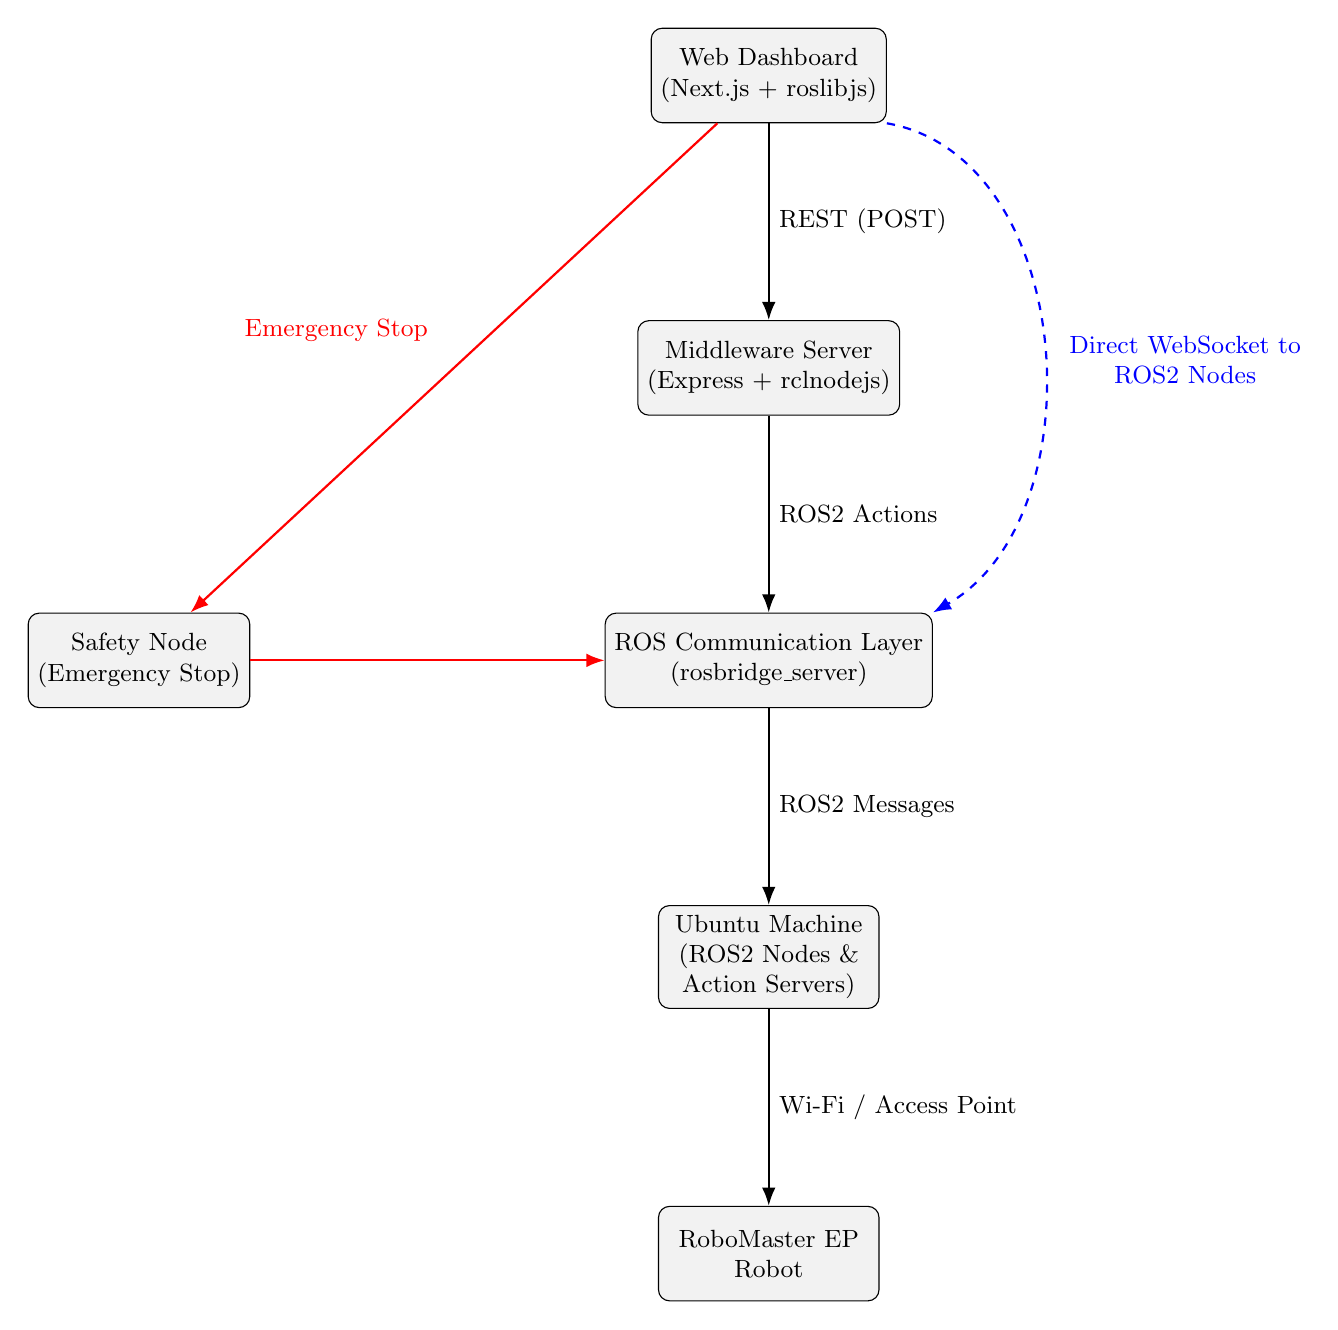
\begin{tikzpicture}[
            node distance=2.5cm and 2.5cm,
            every node/.style={font=\small, align=center},
            box/.style={draw, rounded corners, minimum width=2.8cm, minimum height=1.2cm, fill=gray!10},
            arrow/.style={-Latex, thick}
        ]

        % Nodes
        \node[box] (dashboard) {Web Dashboard\\ (Next.js + roslibjs)};
        \node[box, below=of dashboard] (middleware) {Middleware Server\\ (Express + rclnodejs)};
        \node[box, below=of middleware] (rosbridge) {ROS Communication Layer\\ (rosbridge\_server)};
        \node[box, below=of rosbridge] (ubuntu) {Ubuntu Machine\\ (ROS2 Nodes \&\\ Action Servers)};
        \node[box, below=of ubuntu] (robot) {RoboMaster EP\\ Robot};

        % Connections
        \draw[arrow] (dashboard) -- node[right] {REST (POST)} (middleware);
        \draw[arrow] (middleware) -- node[right] {ROS2 Actions} (rosbridge);
        \draw[arrow] (rosbridge) -- node[right] {ROS2 Messages} (ubuntu);
        \draw[arrow] (ubuntu) -- node[right] {Wi-Fi / Access Point} (robot);

        % Direct connection from dashboard to ubuntu (ROS2 Nodes)
        \draw[arrow, dashed, blue] (dashboard.south east) to[out=-10,in=30] node[right, xshift=2mm, yshift=-2mm, text=blue] {Direct WebSocket to\\ROS2 Nodes} (rosbridge.north east);

        % Emergency stop
        \node[box, left=4.5cm of rosbridge] (safety) {Safety Node\\ (Emergency Stop)};
        \draw[arrow, thick, red] (dashboard) -- node[above left, xshift=-2mm, yshift=2mm, text=red] {Emergency Stop} (safety);
        \draw[arrow, thick, red] (safety) -- (rosbridge);

    \end{tikzpicture}
    \caption{System architecture for Wizard-of-Oz control of the RoboMaster EP robot. The dashboard communicates with the middleware server via REST (POST request), and can also communicate directly with the ROS2 nodes using WebSocket (roslibjs).}
    \label{fig:system-architecture}
\end{figure}

\subsection{\textbf{Dashboard Interface}}
\todo[inline]{
    Here we will describe the final dashboard interface, including the main features and functionalities.
    We will also include screenshots of the dashboard to illustrate its design and layout.
}

\section{\textbf{Usage Research: Formative Evaluation and Iterative Co-Design}}\label{sec:evaluation}
Formative evaluation is a method of assessing a system during its development, with the goal of identifying areas for improvement and guiding the design process from its earliest stages.
In this project, formative evaluation was used as a continuous, participatory method to shape both the interface and the robot's behavioral patterns.
By integrating insights from diverse stakeholders: experts, high school students, and middle school children, the system evolved through iterative feedback.
This approach enabled responsive design decisions and supported the co-creation of meaningful child-robot interaction scenarios.

This section presents the evaluation of the system through three exploratory sessions, each structured as an iterative walkthrough.
These sessions aimed to assess the usability and flexibility of the dashboard, understand the dynamics of child-robot interaction, and collect feedback to inform the design of both the interface and the robot's behavior.
Each evaluation contributed to the co-design process by revealing user needs and contextual challenges in real time.

The sessions included:
(1) a walkthrough with HCI and accessibility experts, who role-played as elementary or middle school students (see Section~\ref{sec:expert-walkthrough});
(2) a session with high school students working in pairs and simulating collaborative behavior on the shared floor mat (see Section~\ref{sec:high-school-walkthrough}); and
(3) a pilot study with middle school children, which evolved into a semi-structured discussion and informal walkthrough focusing on robot behavior and social interaction patterns (see Section~\ref{sec:middle-school-walkthrough}).

The following subsections describe the setup, key observations, and design implications of each session, followed by a summary of the iterative changes implemented in response to user feedback.


\subsection{\textbf{Walkthrough with Experts}}\label{sec:expert-walkthrough}
\subsection*{\textbf{Setup and procedure}}
The first evaluation session was conducted in an office setting and involved two PhD researchers with expertise in Human-Computer Interaction (HCI) and accessibility.
They were asked to role-play as two children collaborating on a Lego tower building task.
Initially, they were seated on the floor approximately one meter apart, with the RoboMaster EP robot placed slightly in front of them at the midpoint of this distance, not directly between them.

The system was operated by an evaluator seated nearby at a desk, with a direct line of sight to the play zone.
A third researcher took notes throughout the session, while two additional observers with expertise in educational technology and human-robot interaction silently monitored the interaction and its outcomes.

Although the scenario was designed around pre-defined robot positions, the participants quickly moved from their initial spots, rendering the static positions ineffective.
However, the dashboard's joystick feature enabled the operator to adapt in real time by manually repositioning the robot and triggering actions.
The session unfolded as a dynamic and playful interaction between the two participants and the robot, including episodes of joint play, interaction breakdowns, and regulatory robot interventions.

After the active session, all participants engaged in an open-ended discussion, which yielded critical reflections on the interface's design, the robot's perceived role, and the effectiveness of various robot behaviors.
These observations and insights directly informed the next iteration of the dashboard.

\subsection*{\textbf{Key observations}}
\begin{itemize}
    \item The pre-defined movement positions were quickly invalidated when the "children" moved from their expected spots. The experts stressed the importance of allowing the operator to improvise and react dynamically.
    \item Negative robot feedback, such as "shaking the head" by spinning on the spot, was perceived as entertaining, rather than corrective. This could encourage children to misbehave just to see the robot react.
    \item Experts observed that opening the box with the gripper and presenting it to a participant invited them to place something inside. This could be used as a form of collaborative engagement or de-escalation.
    \item Experts emphasized the importance of distinguishing between different levels of feedback, both positive and negative.
          For positive reinforcement, a scalable approach could include combinations of lights, sounds, and movement, ranging from a simple LED blink to a celebratory motion sequence.
          Negative feedback, on the other hand, should be kept minimal and neutral: limited to red lights, with no sound, and little to no movement, possibly just a slight backward motion to signal withdrawal.
          Sound should be excluded from negative interventions entirely to prevent the robot from becoming a source of entertainment.
    \item The robot was perceived more as a "peer" than an authority figure, prompting the need to frame it accordingly in both behavior and design.
    \item Experts advised against focusing the robot's attention too much on one child, as this could lead to perceptions of unfairness.
    \item Introducing the robot to children before the task might help reduce distractions during the experiment, as curiosity would be partially satisfied beforehand.
    \item Large Lego Duplo bricks limited complexity of the task; smaller pieces might offer a more engaging challenge.
\end{itemize}

\subsection*{\textbf{Design implications}}
The insights from this session led to a clear shift in the robot's perceived role: its behavior was intentionally designed to be cooperative, inclusive, and friendly, reinforcing its identity as a peer rather than a disciplinarian.
Feedback modalities were explicitly separated into positive and negative categories to avoid ambiguity, with sound reserved only for positive reinforcement.
The dashboard was enhanced to grant the operator broader and more flexible control over the robot, including nuanced gripper manipulation and advanced LED configurations such as customizable colors, blink timing, and speed.
The importance of joystick-based improvisation was validated, ensuring the operator could dynamically adapt to unpredictable child behavior.
Overall, these refinements improved both the responsiveness and expressiveness of the system, aligning robot actions more closely with user expectations and the playful, peer-like framing advocated by the experts.

\subsection{\textbf{Walkthrough with High School Students}}\label{sec:high-school-walkthrough}
\subsection*{\textbf{Setup and procedure}}
The second evaluation session was conducted in a spacious conference room.
A large children's floor mat was added to define a playful zone, following recommendations from the first experiment.
The robot used the updated Version 2 of the dashboard interface, which incorporated changes such as feedback intensity levels and different LED color options.

The session involved four high school students, divided into two pairs.
Each pair was asked to role-play as younger children (elementary or middle school age) participating in a turn-taking Lego activity.
The robot was operated by an evaluator from a nearby desk.
Before the session began, the robot was introduced to the participants to reduce initial distraction, another refinement based on the previous walkthrough.

Each pair of students participated in two stages:
\begin{itemize}
    \item \textbf{Step 1: Robot as Regulator} - The two "children" were asked to collaborate on building a Lego tower while occasionally engaging in simulated turn-taking violations.
          The robot was expected to intervene using visual and movement-based feedback.
    \item \textbf{Step 2: Child as Regulator} - One student built a Lego structure with help from the robot, while the second student acted as a mediator.
          The robot would occasionally behave incorrectly (e.g., bringing the wrong Lego piece or running away), prompting the mediator to "teach" the robot how to behave, following the Learning by Teaching paradigm.
    \item \textbf{Step 3: Co-Design Discussion} - After the interaction tasks, students were invited to openly discuss their experience with the robot, suggest new behaviors, and reflect on what they would expect from a social robot in this context.
          The session was semi-structured and aimed at eliciting child-led ideas to inform future iterations.
\end{itemize}

The same three-stage procedure was repeated with the second pair of students.
During the first round, all four students were present and participated in observing or acting.
However, for the second round, only the second pair remained, as the first group had to leave the session early due to other commitments.

\subsection*{\textbf{Key observations}}
\begin{itemize}
    \item Red LED signals alone were insufficient to attract attention, especially due to ambient lighting and the robot's position on the floor.
    \item The lack of sound in negative feedback led to the robot being ignored during turn-taking violations. Participants were focused on the Lego task and did not notice subtle visual cues.
    \item A more effective attention-grabbing strategy was to have the robot "invade" the children's personal space with a quick approach motion.
    \item The robot being named by the students helped increase its perceived presence and relational value during interactions.
    \item One participant suggested that the robot could turn around and "walk away" when reacting negatively, simulating being upset or "offended."
\end{itemize}

\subsection*{\textbf{Design implications}}
Observations from this walkthrough demonstrated that visual cues alone were often insufficient to capture attention, particularly when the robot was positioned on the floor.
To address this, movement-based feedback was amplified, with more pronounced and even slightly intrusive motions, such as quick approaches or turning away, used to reinforce the robot's presence and personality.
The practice of letting children name the robot was recognized as a valuable means of enhancing engagement and relational dynamics, especially in scenarios involving repeated or long-term interaction.
These findings validated the flexible and expressive behavior options introduced after the expert walkthrough, and led to further interface refinements, such as the addition of more LED color choices to support clearer signaling during tasks that required specific requests.
The overall design thus became more attuned to real-world interaction needs and child-driven engagement.

\subsection{\textbf{Walkthrough with Middle School Students}}\label{sec:middle-school-walkthrough}
\subsection*{\textbf{Setup and procedure}}
The final evaluation session was conducted in the same spacious conference room used in the previous walkthrough.
A children's floor mat was again placed at the center of the space, but this time smaller Lego bricks were provided to increase task flexibility and challenge.
The robot was operated using the final version of the dashboard interface.
Three girls who had recently started middle school participated in the session.
They were told beforehand that the experiment was a Wizard-of-Oz setup, and the robot was introduced at the beginning of the session to help mitigate distractions.

The team consisted of the operator, an observing researcher, and an additional facilitator who sat on the floor with the participants, guiding them through each experimental step and prompting them for feedback.
The session followed the same structure as previous walkthroughs but was run with all three children at the same time.

\begin{itemize}
    \item \textbf{Step 1: Robot as Regulator} - The children were asked to collaboratively build a Lego tower while occasionally breaking the turn-taking rule.
          The robot attempted to intervene using lights, movement, and audio cues.
          However, the feedback signals were often ignored or went unnoticed due to high ambient noise and the robot's position on the floor.
    \item \textbf{Step 2: Child as Regulator} - Two children played with the robot while the third acted as a regulator.
          The robot sometimes performed incorrect or disruptive actions (e.g., stealing pieces or pretending to help but failing), prompting the regulator to guide or correct the behavior.
          The robot responded with positive or negative signals based on this guidance.
    \item \textbf{Step 3: Social Behavior and Emotion Teaching} - In a final interaction, children were asked to teach the robot about concepts like personal space, polite requesting, and emotional understanding.
          The robot performed incorrect distances or behaviors, prompting the children to explain or demonstrate appropriate actions.
\end{itemize}

\subsection*{\textbf{Key observations}}
\begin{itemize}
    \item The robot continued to be perceived more as a pet (e.g., a dog) than as a peer or authority figure, reinforcing previous observations.
    \item Children named the robot and began interacting with it socially, including petting it on the box/head and decorating it with Lego bricks.
    \item Visual feedback like LEDs remained mostly ineffective; participants suggested that a table-based setup could raise the robot to eye level and improve visibility.
    \item Fast and unpredictable movements were effective at capturing attention, sometimes even surprising the participants.
    \item Positive feedback involving lights, sound, and movement ("dances") was appreciated and engaging.
    \item Participants showed strong interest in how the robot could recognize human emotions and tailor its behavior accordingly.
    \item During Step 2, children experimented with rewarding the robot for good behavior, and teaching it when to stop disruptive actions.
    \item In Step 3, they proposed using facial expressions, tone of voice, and environmental context to assess emotions and social cues.
    \item They also expressed a desire for the robot to have an onboard interface to communicate or show its own internal emotional state.
    \item After extended time with the robot (over one hour), the children continued to engage with it playfully while discussing social and emotional aspects.
\end{itemize}

\subsection*{\textbf{Design implications}}
The findings from this session highlighted the importance of acknowledging the robot's perceived identity, as children consistently related to it more as a pet-like companion than as a peer or authority figure.
This insight informed the ongoing design by encouraging the use of playful, multimodal feedback, combining lights, sound, and expressive movement, with the intensity of cues scaled to the importance of the situation.
Suggestions to improve the visibility of visual signals, such as elevating the robot or adding auxiliary displays, were considered to address the limitations of floor-based interactions.
Furthermore, the children's enthusiasm for emotional awareness features, like interpreting tone of voice, facial expressions, and proximity, pointed toward future enhancements in autonomous behavior and social context sensitivity.
The idea of equipping the robot with an on-device interface also emerged as a promising direction for enabling more direct, child-driven communication and mutual understanding.
Overall, co-design insights from this session reinforced the value of tailoring robot behavior to both the social context and the emotional landscape of the interaction.

\subsection{\textbf{Summary of Iterative Design Changes}}
This section summarizes the key iterative changes that shaped both the dashboard interface and the robot's behavior across the three evaluation sessions.
Each walkthrough revealed new user needs and inspired concrete refinements.
Interface updates were driven by usability and expressiveness goals, while behavioral adaptations emerged through co-design discussions and observational insights.
Screenshots of the evolving interface are included to illustrate the progression from the initial prototype to the final deployed version.

\subsubsection*{\textbf{Version 1 - Initial Prototype}}
\begin{itemize}
    \item Basic joystick and pre-defined movement controls.
    \item Minimal bad-behavior feedback capabilities (red LED, spin, sound).
    \item No dedicated gripper control (box could only be opened/closed by moving the arm); no feedback intensity levels.
\end{itemize}
\begin{figure}[H]
    \centering
    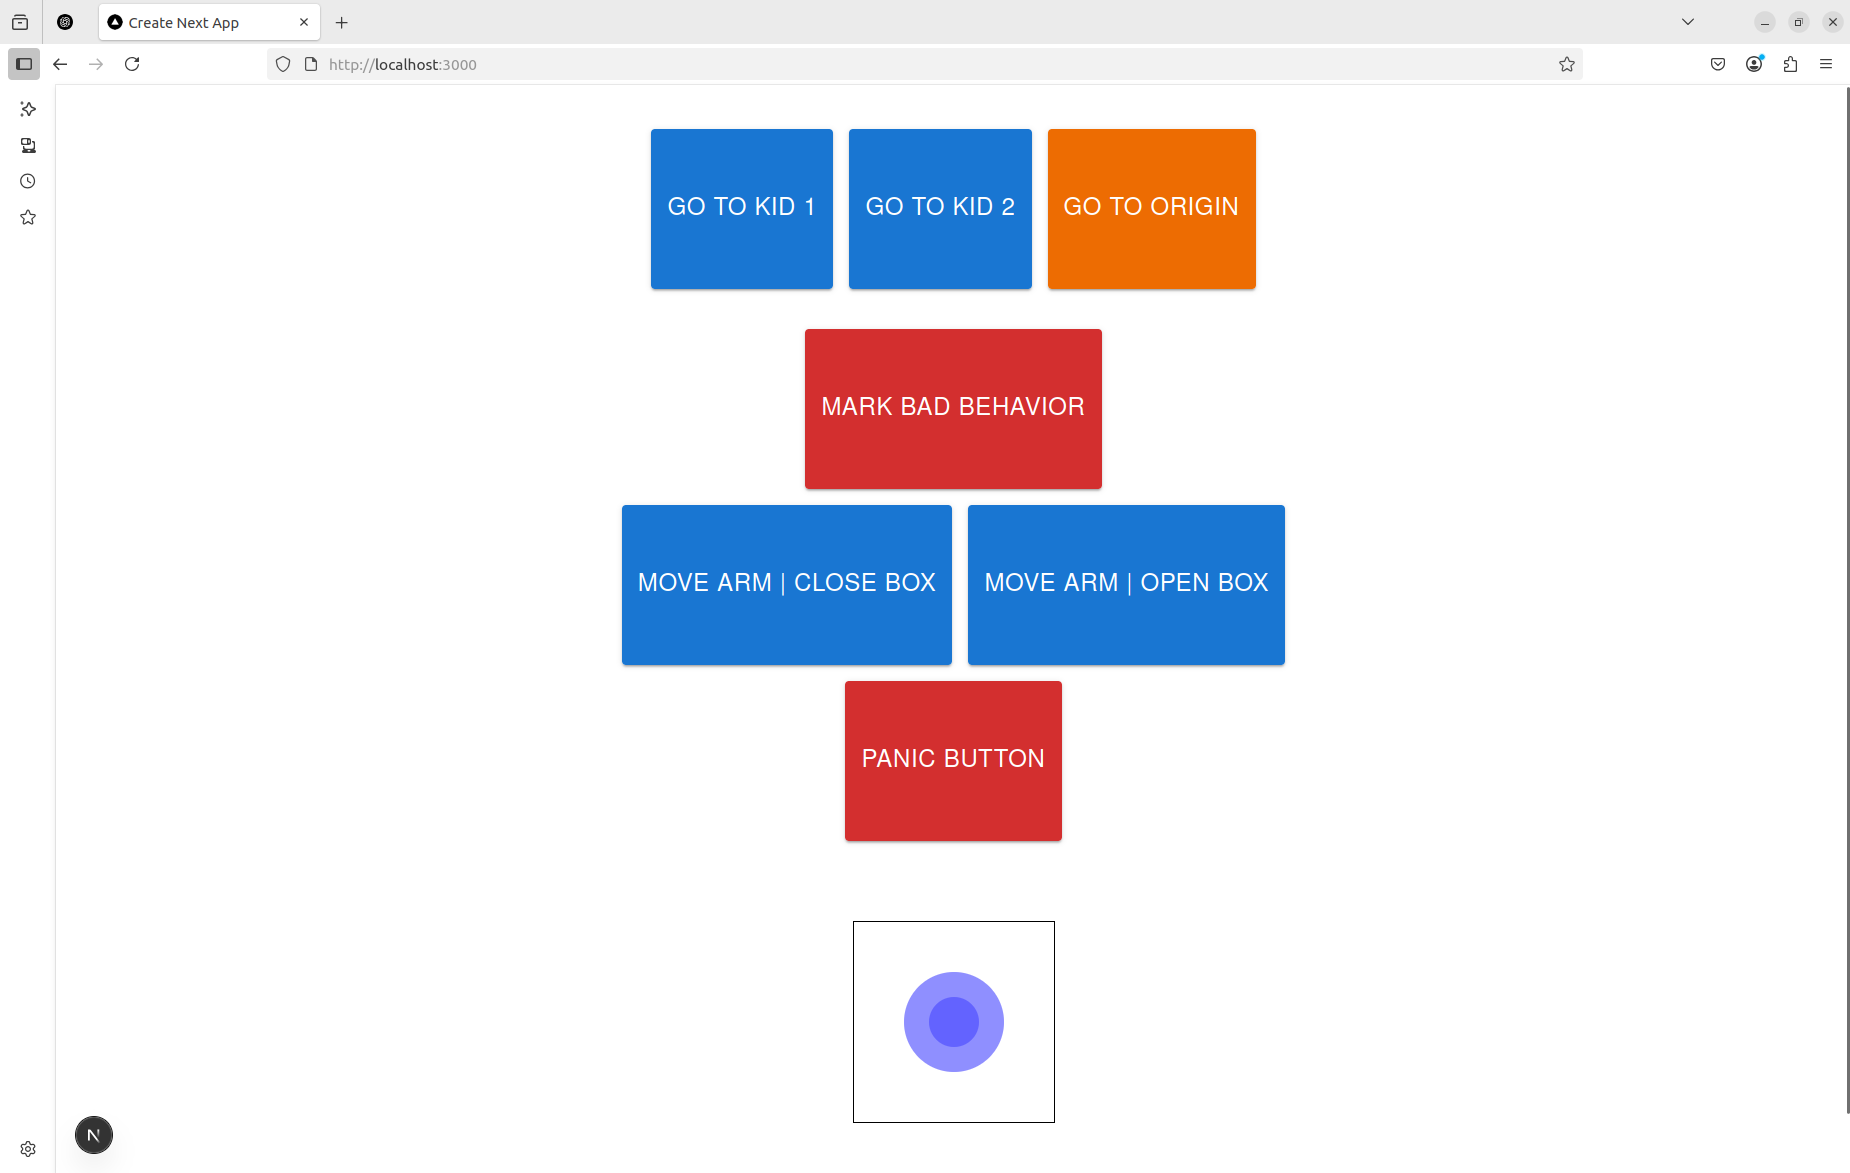
\includegraphics[width=0.8\linewidth]{figures/dashboard_v1.png}
    \caption{Version 1 - Initial prototype with limited robot control and feedback options.}
    \label{fig:dashboard-v1}
\end{figure}

\subsubsection*{\textbf{Version 2 - Post Expert Walkthrough}}
\begin{itemize}
    \item Added gripper controls and advanced LED configuration (colors, blink timing, speed).
    \item Introduced feedback modes: positive and negative with scalable intensity.
    \item Refined movement control and added panic button.
    \item Macro-scenarios for quick intervention.
    \item UI layout was reorganized into functional panels or "zones" to streamline operator access to robot features.
\end{itemize}
\begin{figure}[H]
    \centering
    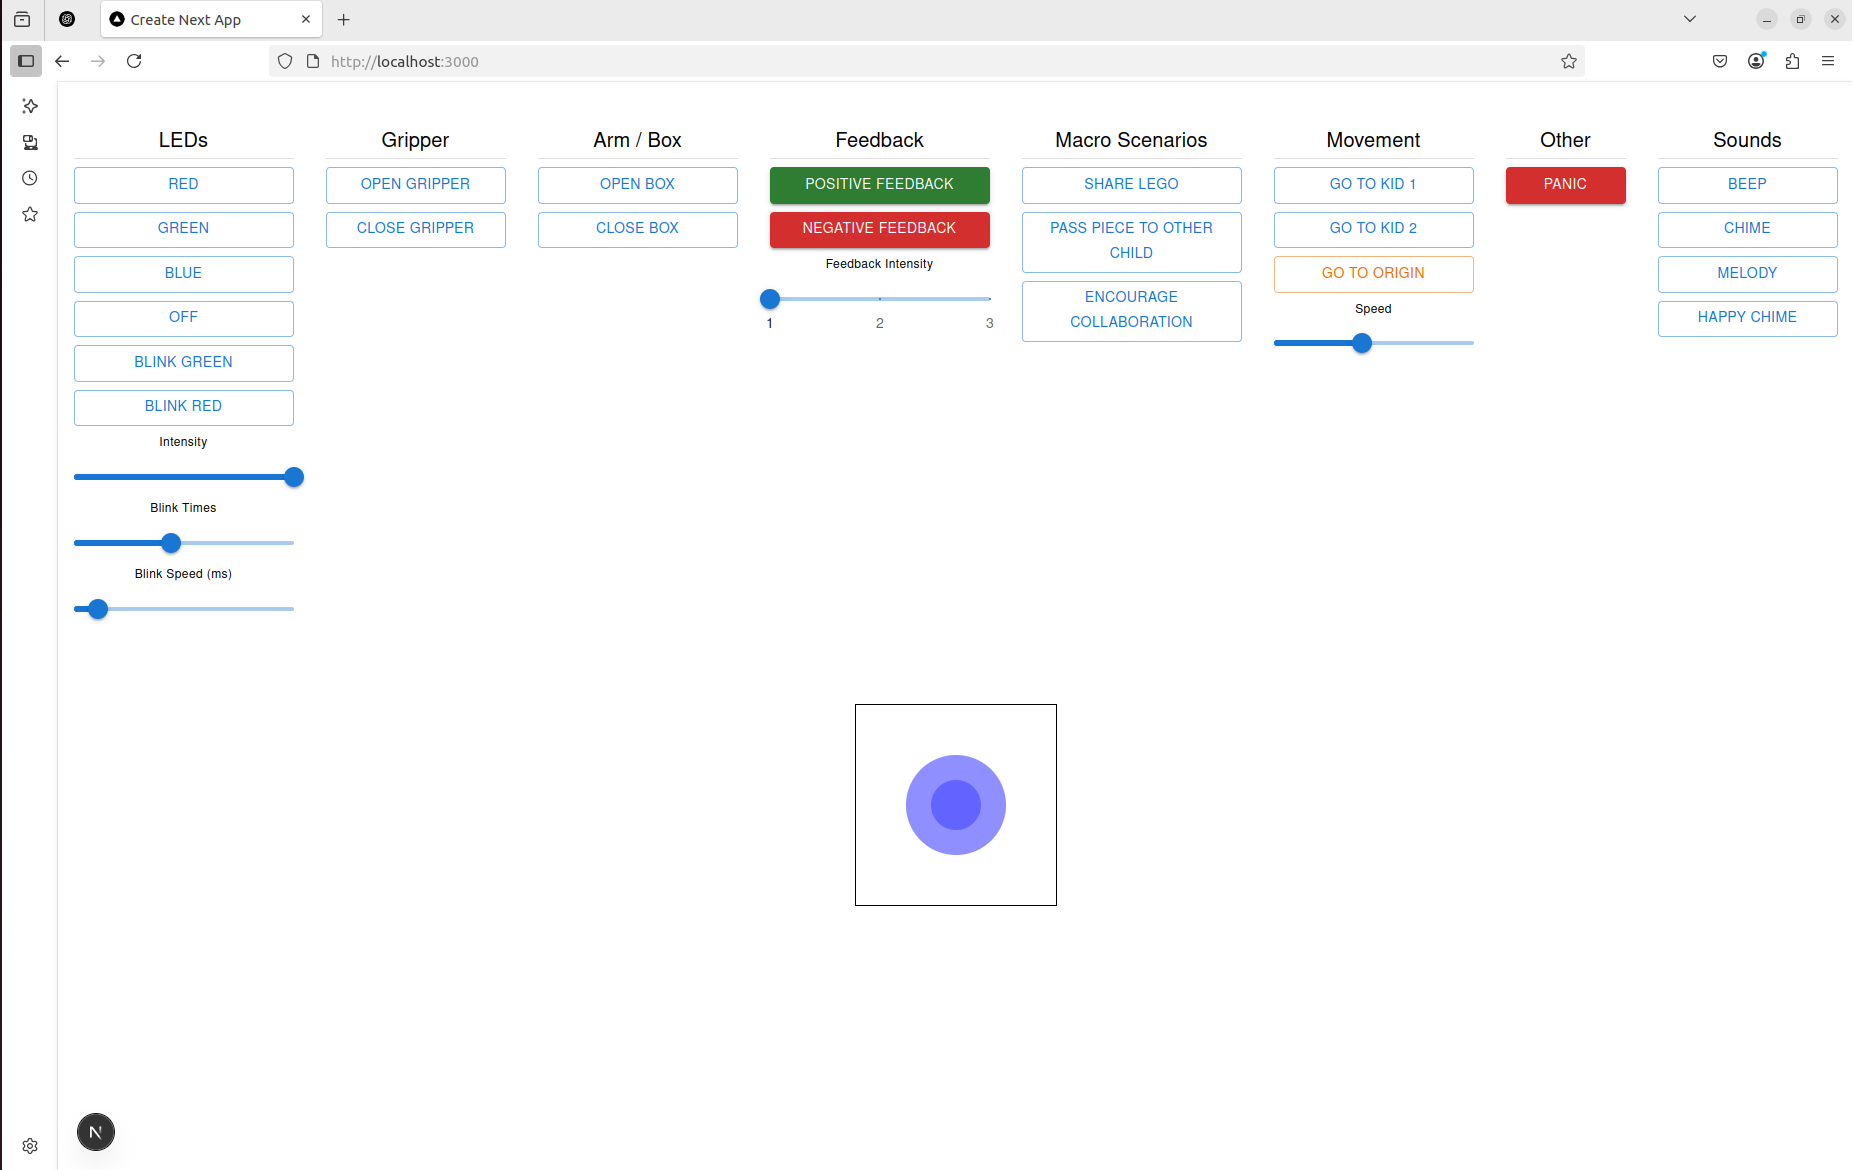
\includegraphics[width=0.8\linewidth]{figures/dashboard_v2.png}
    \caption{Version 2 - Refined interface after expert feedback, supporting greater flexibility.}
    \label{fig:dashboard-v2}
\end{figure}

\subsubsection*{\textbf{Version 3 - Final Version for Pilot Study}}
\begin{itemize}
    \item Further expanded LED signaling options for color-specific communication.
    \item Audio feedback support for positive cues only.
    \item Increased the size and visual prominence of the panic button to improve operator responsiveness during high-pressure scenarios.
\end{itemize}
\begin{figure}[H]
    \centering
    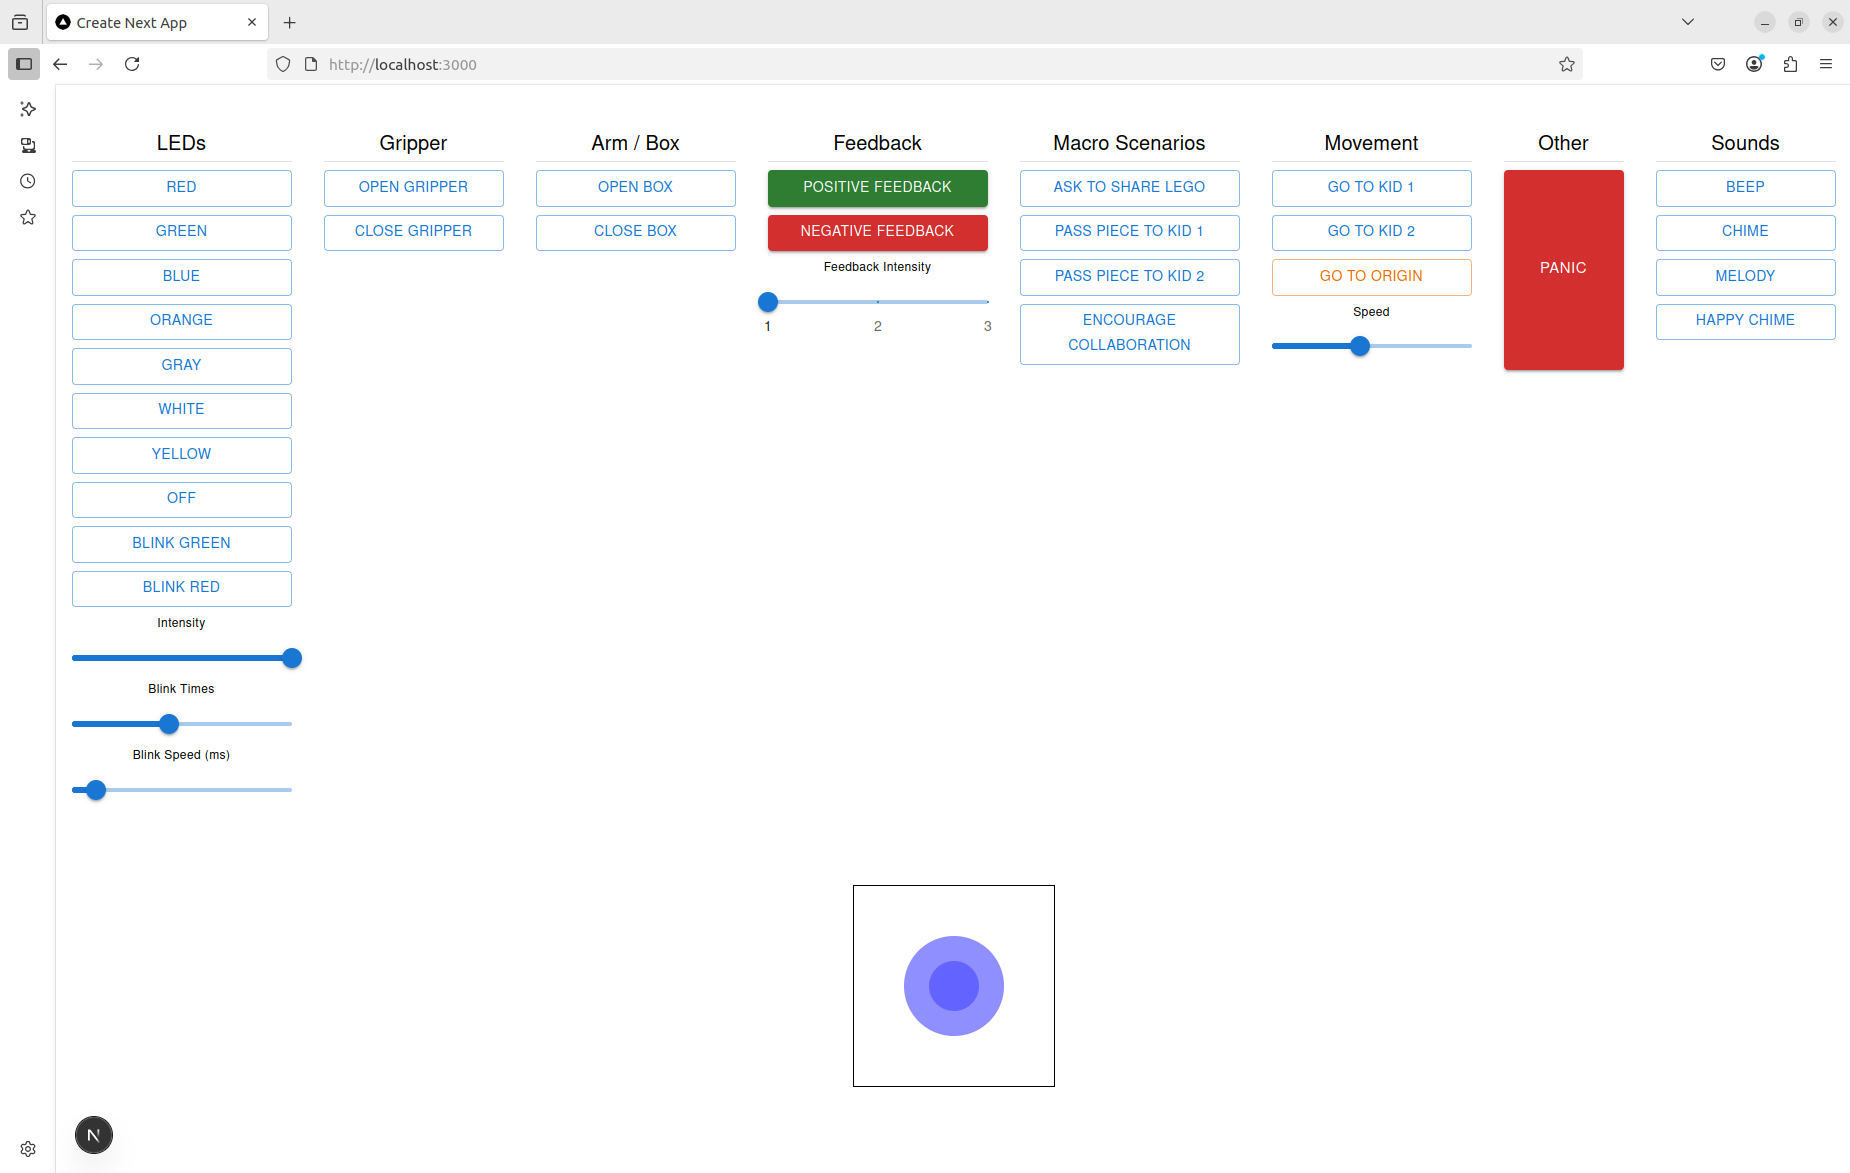
\includegraphics[width=0.8\linewidth]{figures/dashboard_v3.png}
    \caption{Version 3 - Final dashboard interface used in the pilot experiment.}
    \label{fig:dashboard-v3}
\end{figure}

\subsection{\textbf{Behavioral Design Iterations}}

Beyond interface adjustments, each walkthrough also shaped our understanding of effective robot behaviors in child-facing settings.

Across the three walkthroughs, a consistent pattern emerged in how children and experts responded to the robot's behavior.
Rather than detailing new robot actions, participants influenced the style, tone, and social framing of these actions, shifting the robot from an authority figure to a pet-like peer.
This shift affected the design of feedback modalities (e.g., neutral negative feedback, celebratory positive feedback) and the narrative framing of the robot within the experiment.
These reflections did not result in autonomous learning, but they directly shaped the robot's available actions and responses,
expanding its behavioral repertoire and enabling the operator to deliver more socially aligned interventions.
This iterative refinement represented one of the three core directions explored throughout the experiments and laid the groundwork for Step 3 of the study,
where the robot begins to apply these socially informed behaviors in response to interaction cues.
While still operator-driven, this stage anticipates future developments toward semi-autonomous behavior grounded in prior human-led interventions (see Section~\ref{sec:design}).
\\
Key insights included:
\begin{itemize}
    \item \textbf{Framing of the Robot:} Children consistently perceived the robot as a playful companion or pet, rather than an authority figure.\\
          This influenced design decisions toward peer-like, non-disciplinary behaviors. [Exp 1--3]
    \item \textbf{Feedback Intensity:} Both experts and children emphasized the importance of scalable, multimodal feedback (e.g., lights + movement + sound), especially for positive interactions.\\
          Negative feedback should remain neutral and minimal to avoid encouraging misbehavior. [Exp 1--3]
    \item \textbf{Social Engagement:} Naming the robot, petting it, and attributing personality to it emerged naturally, suggesting personalization features may enhance engagement. [Exp 2--3]
    \item \textbf{Learning by Teaching:} Children actively guided the robot using verbal and physical cues, validating the LbT framing.\\
          Tasks like teaching the robot to maintain distance or follow polite commands proved intuitive and effective. [Exp 2--3]
    \item \textbf{Emotion and Context Awareness:} Middle school students suggested that robots should use emotional cues, facial expressions, and context to decide how and when to interact. [Exp 3]
\end{itemize}

These behavioral reflections informed the structure of robot actions available through the dashboard, highlighting design directions for future exploration of semi-autonomous and emotionally aware systems.

\newpage

\section{\textbf{Conclusions}}\label{sec:conclusions}
This project presents the design and implementation of a web-based dashboard to enable Wizard-of-Oz control of a social robot used in a Learning by Teaching experiment with children.
The system is part of the larger TESORO initiative and lays the groundwork for studying how social robots can assist in learning soft skills like turn-taking.
\todo[inline]{To be expanded}

\subsection{\textbf{Future Work}}
\todo[inline]{
    Here we will write about future work like the ones mentioned in the TESORO project proposal like :
    Long-term goal: enabling real-time learning from the child's regulatory actions and shifting toward semi-autonomous robot behavior.
}


%%%%% BIBLIOGRAPHY %%%%%
\bibliographystyle{abbrv}
\bibliography{references}

\end{document}
